\uuid{IMXU}
\exo7id{7378}
\titre{exo7 7378}
\auteur{mourougane}
\organisation{exo7}
\datecreate{2021-08-10}
\isIndication{false}
\isCorrection{true}
\chapitre{Groupe, anneau, corps}
\sousChapitre{Autre}
\module{Algèbre}
\niveau{L2}
\difficulte{}

\contenu{
\texte{

}
\begin{enumerate}
    \item \question{Sur le cercle unité, on a marqué les éléments du groupe des racines de l'unité d'ordre $8$. Soit
$\zeta = \exp(2i \pi/8)$.
Représenter sur un cercle unité les éléments du sous-groupe engendré par~$\zeta^3$.}
\reponse{Comme $\zeta$ est d'ordre $8$, $\zeta^3$ est d'ordre 
$8/\pgcd(8,3)=8$. Le sous-groupe engendré par $\zeta^3$ est donc tout le groupe des racines de l'unité d'ordre $8$.

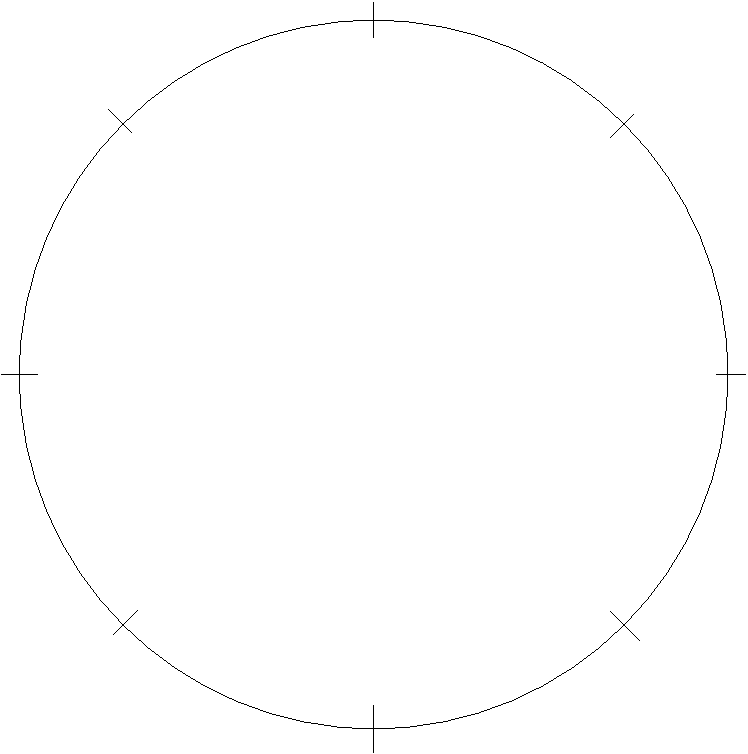
\includegraphics[scale=0.7]{images/img-mour-130}}
    \item \question{Soit la racine de l'unité $z = \exp(16 i \pi/11)$. 
Déterminer son ordre dans le groupe $\C^\star$.
Déterminer l'ordre de $z^8$. Déterminer l'argument de $z^8$.}
\reponse{$z^11=1$ donc l'ordre de $z$ est un diviseur de $11$. Mais $z\not=1$. Donc $z$ est d'ordre $11$.
Comme $z^8\not=1$, $z^8$ est aussi d'ordre $11$.
$z^8=\exp(16\times 8 i \pi/11)=\exp(64\times 2i \pi/11)$.
Comme $64=5\times 11+9$, l'argument de $z^8$ est $18\pi/11$.}
\end{enumerate}
}
